\section{Các lượt quét siêu tham số còn lại}
\label{app:sweeps}
\begin{figure}[H]
\centering
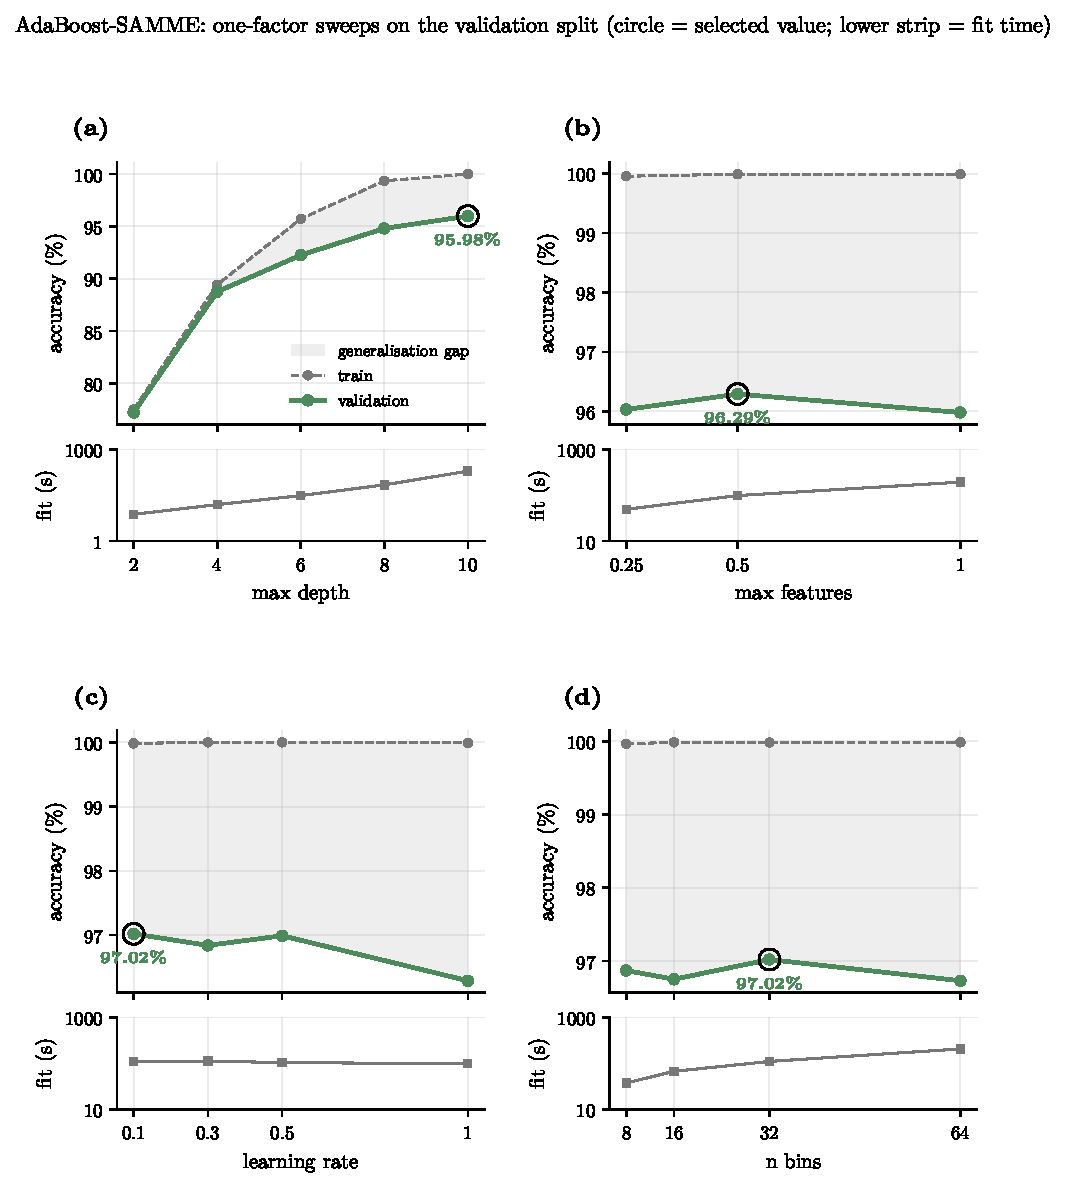
\includegraphics[width=0.9\textwidth]{../results/figures/sweep_adaboost.pdf}
\caption{AdaBoost-SAMME: quét từng siêu tham số trên validation (số vòng boosting chọn riêng từ đường cong, \cref{fig:curves}c).}
\end{figure}
\begin{figure}[H]
\centering
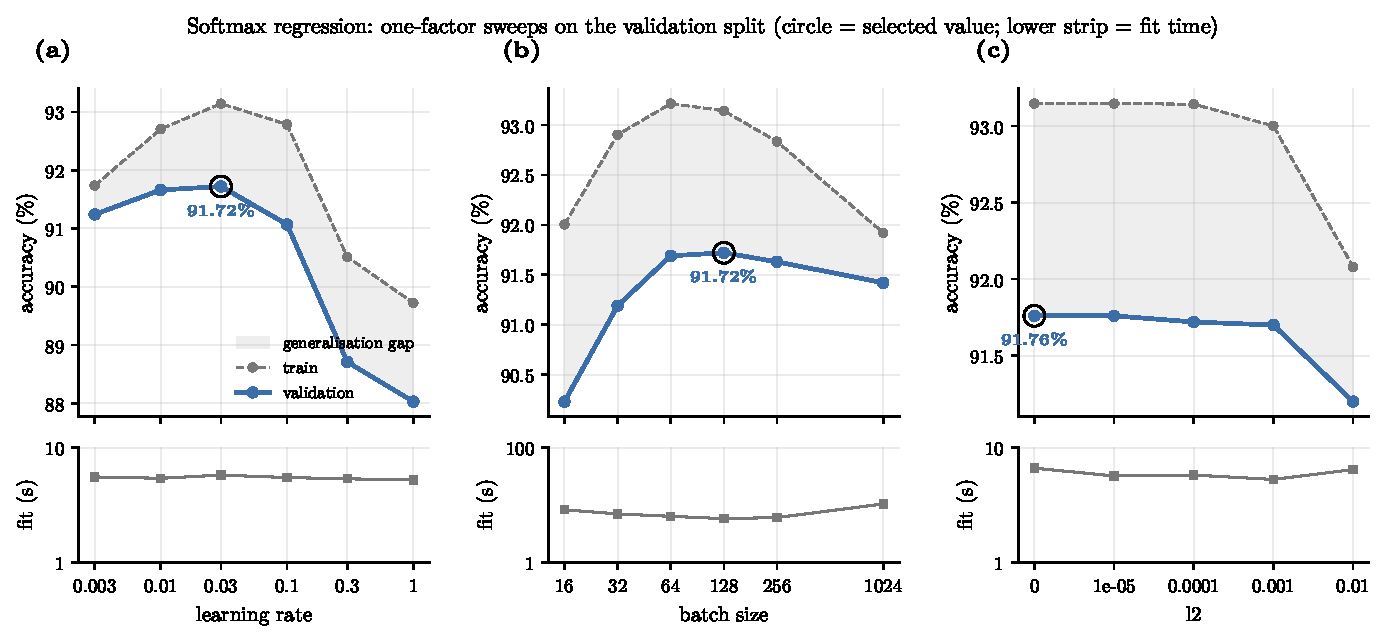
\includegraphics[width=0.9\textwidth]{../results/figures/sweep_softmax.pdf}
\caption{Hồi quy softmax: quét từng siêu tham số trên validation.}
\end{figure}
\begin{figure}[H]
\centering
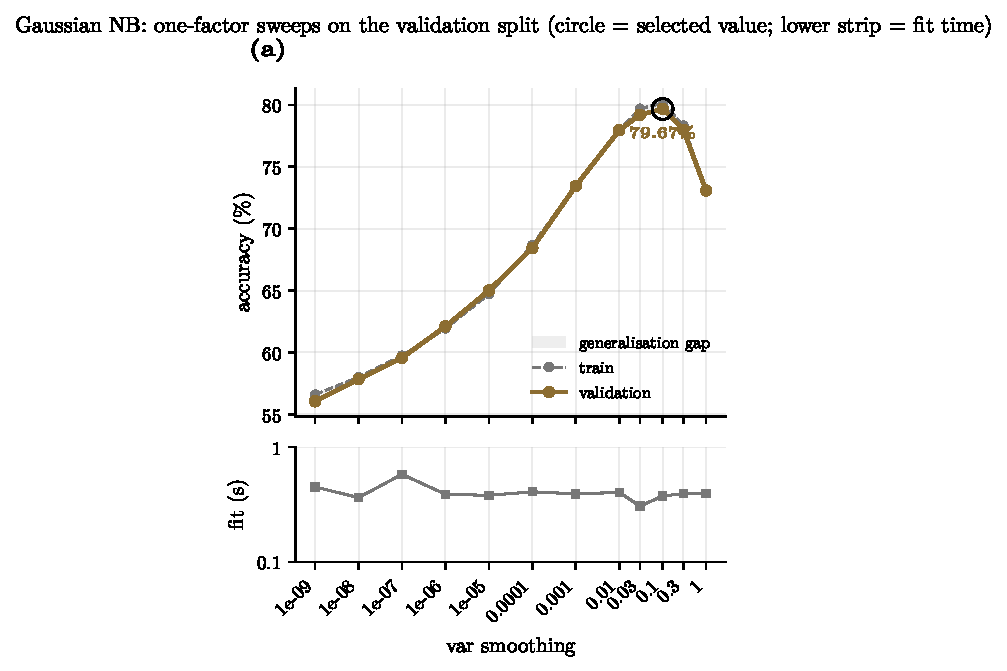
\includegraphics[width=0.45\textwidth]{../results/figures/sweep_naive_bayes.pdf}
\caption{Gaussian Naïve Bayes: quét \texttt{var\_smoothing} trên validation.}
\end{figure}

\section{Tái lập kết quả}
Môi trường dùng \texttt{uv} (Python $\ge3.11$); mã, kiểm thử và dòng lệnh nằm trong kho GitHub của đồ án.
\begin{verbatim}
uv sync --extra track --extra export
uv run python -m src prepare          # tải MNIST, chia train/val, chuẩn hóa
uv run python -m src tune --model all # quét siêu tham số, ghi results/tuning
uv run python -m src train --model all
uv run python -m src baselines --model all   # scikit-learn
uv run python -m src augment          # thí nghiệm tăng cường dữ liệu
uv run python -m src report           # bảng, hình, các đoạn LaTeX
uv run python -m src export           # ONNX + kiểm tra số học
uv run python -m src upload           # đẩy lên Hugging Face (cần token)
uv run pytest
\end{verbatim}
Báo cáo biên dịch bằng \texttt{pdflatex} + \texttt{bibtex} trong thư mục \texttt{report/}; các bảng và số liệu nằm trong \texttt{results/tables} và \texttt{report/generated} do bước \texttt{report} sinh ra.
